\section{last}

\begin{frame}
    \frametitle{总结与展望}
    % 主要工作:

    % \begin{itemize}
    %     \item 特定结构构造与优化方法研究
    %     \begin{itemize}
    %         \item 基于卷积结构的SDNN预测模型构造与优化方法
    %         \item 基于循环结构的SDNN预测模型构造与优化方法
    %     \end{itemize}
    %     \item 一般结构优化方法研究
    %   \begin{itemize}
    %         \item SDNN预测模型的二重特征结构选择方法
    %     \end{itemize}
    %     \item 混合结构优化方法研究
    %     \begin{itemize}
    %         \item SDNN预测模型的混合结构生长与优化方法
    %     \end{itemize}
    % \end{itemize}
    \begin{figure}[!t]
        \begin{minipage}{0.45\textwidth}
            \centering
            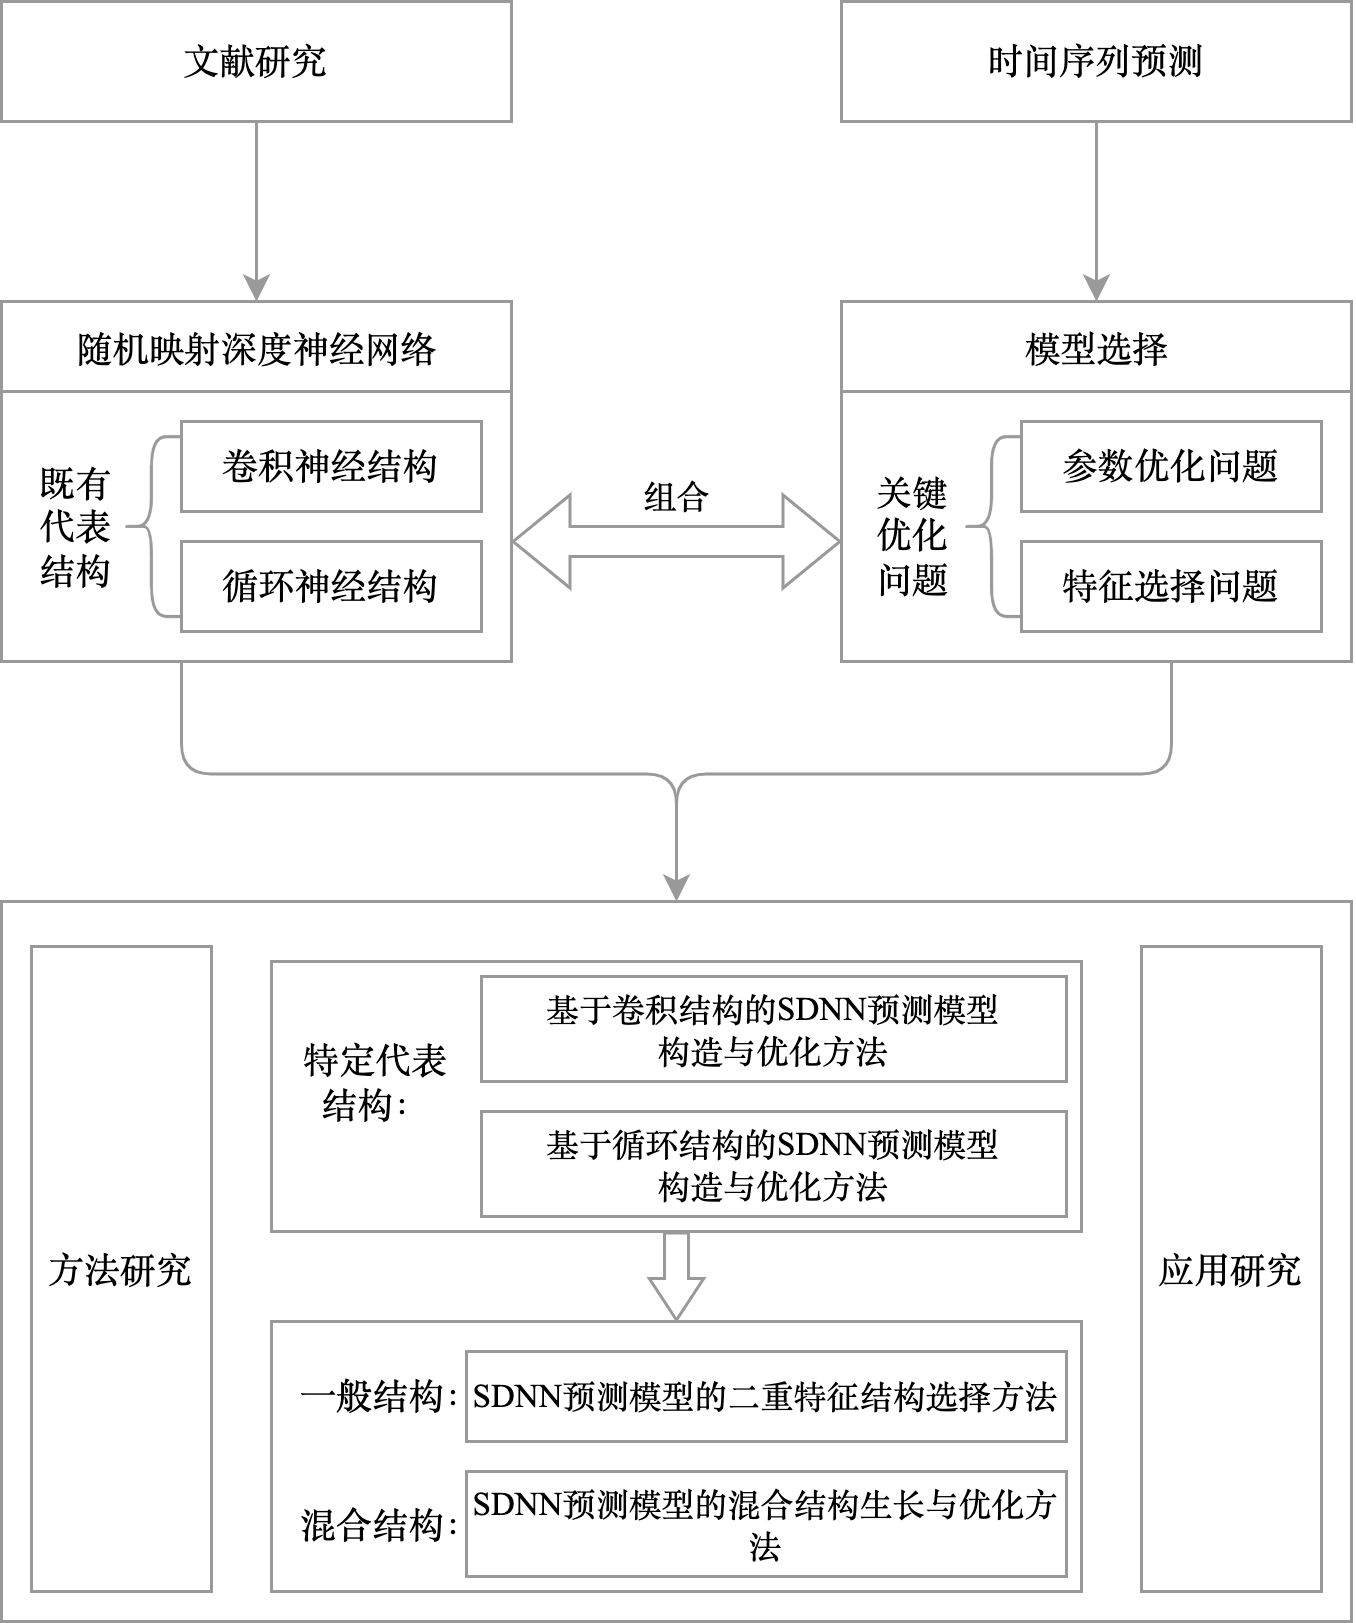
\includegraphics[width=0.825\linewidth]{float/ch.intro/thesis_arch.png}
            \caption*{本研究技术路线}
        \end{minipage}
        \hfill
        \begin{minipage}{0.45\textwidth}
            \centering
            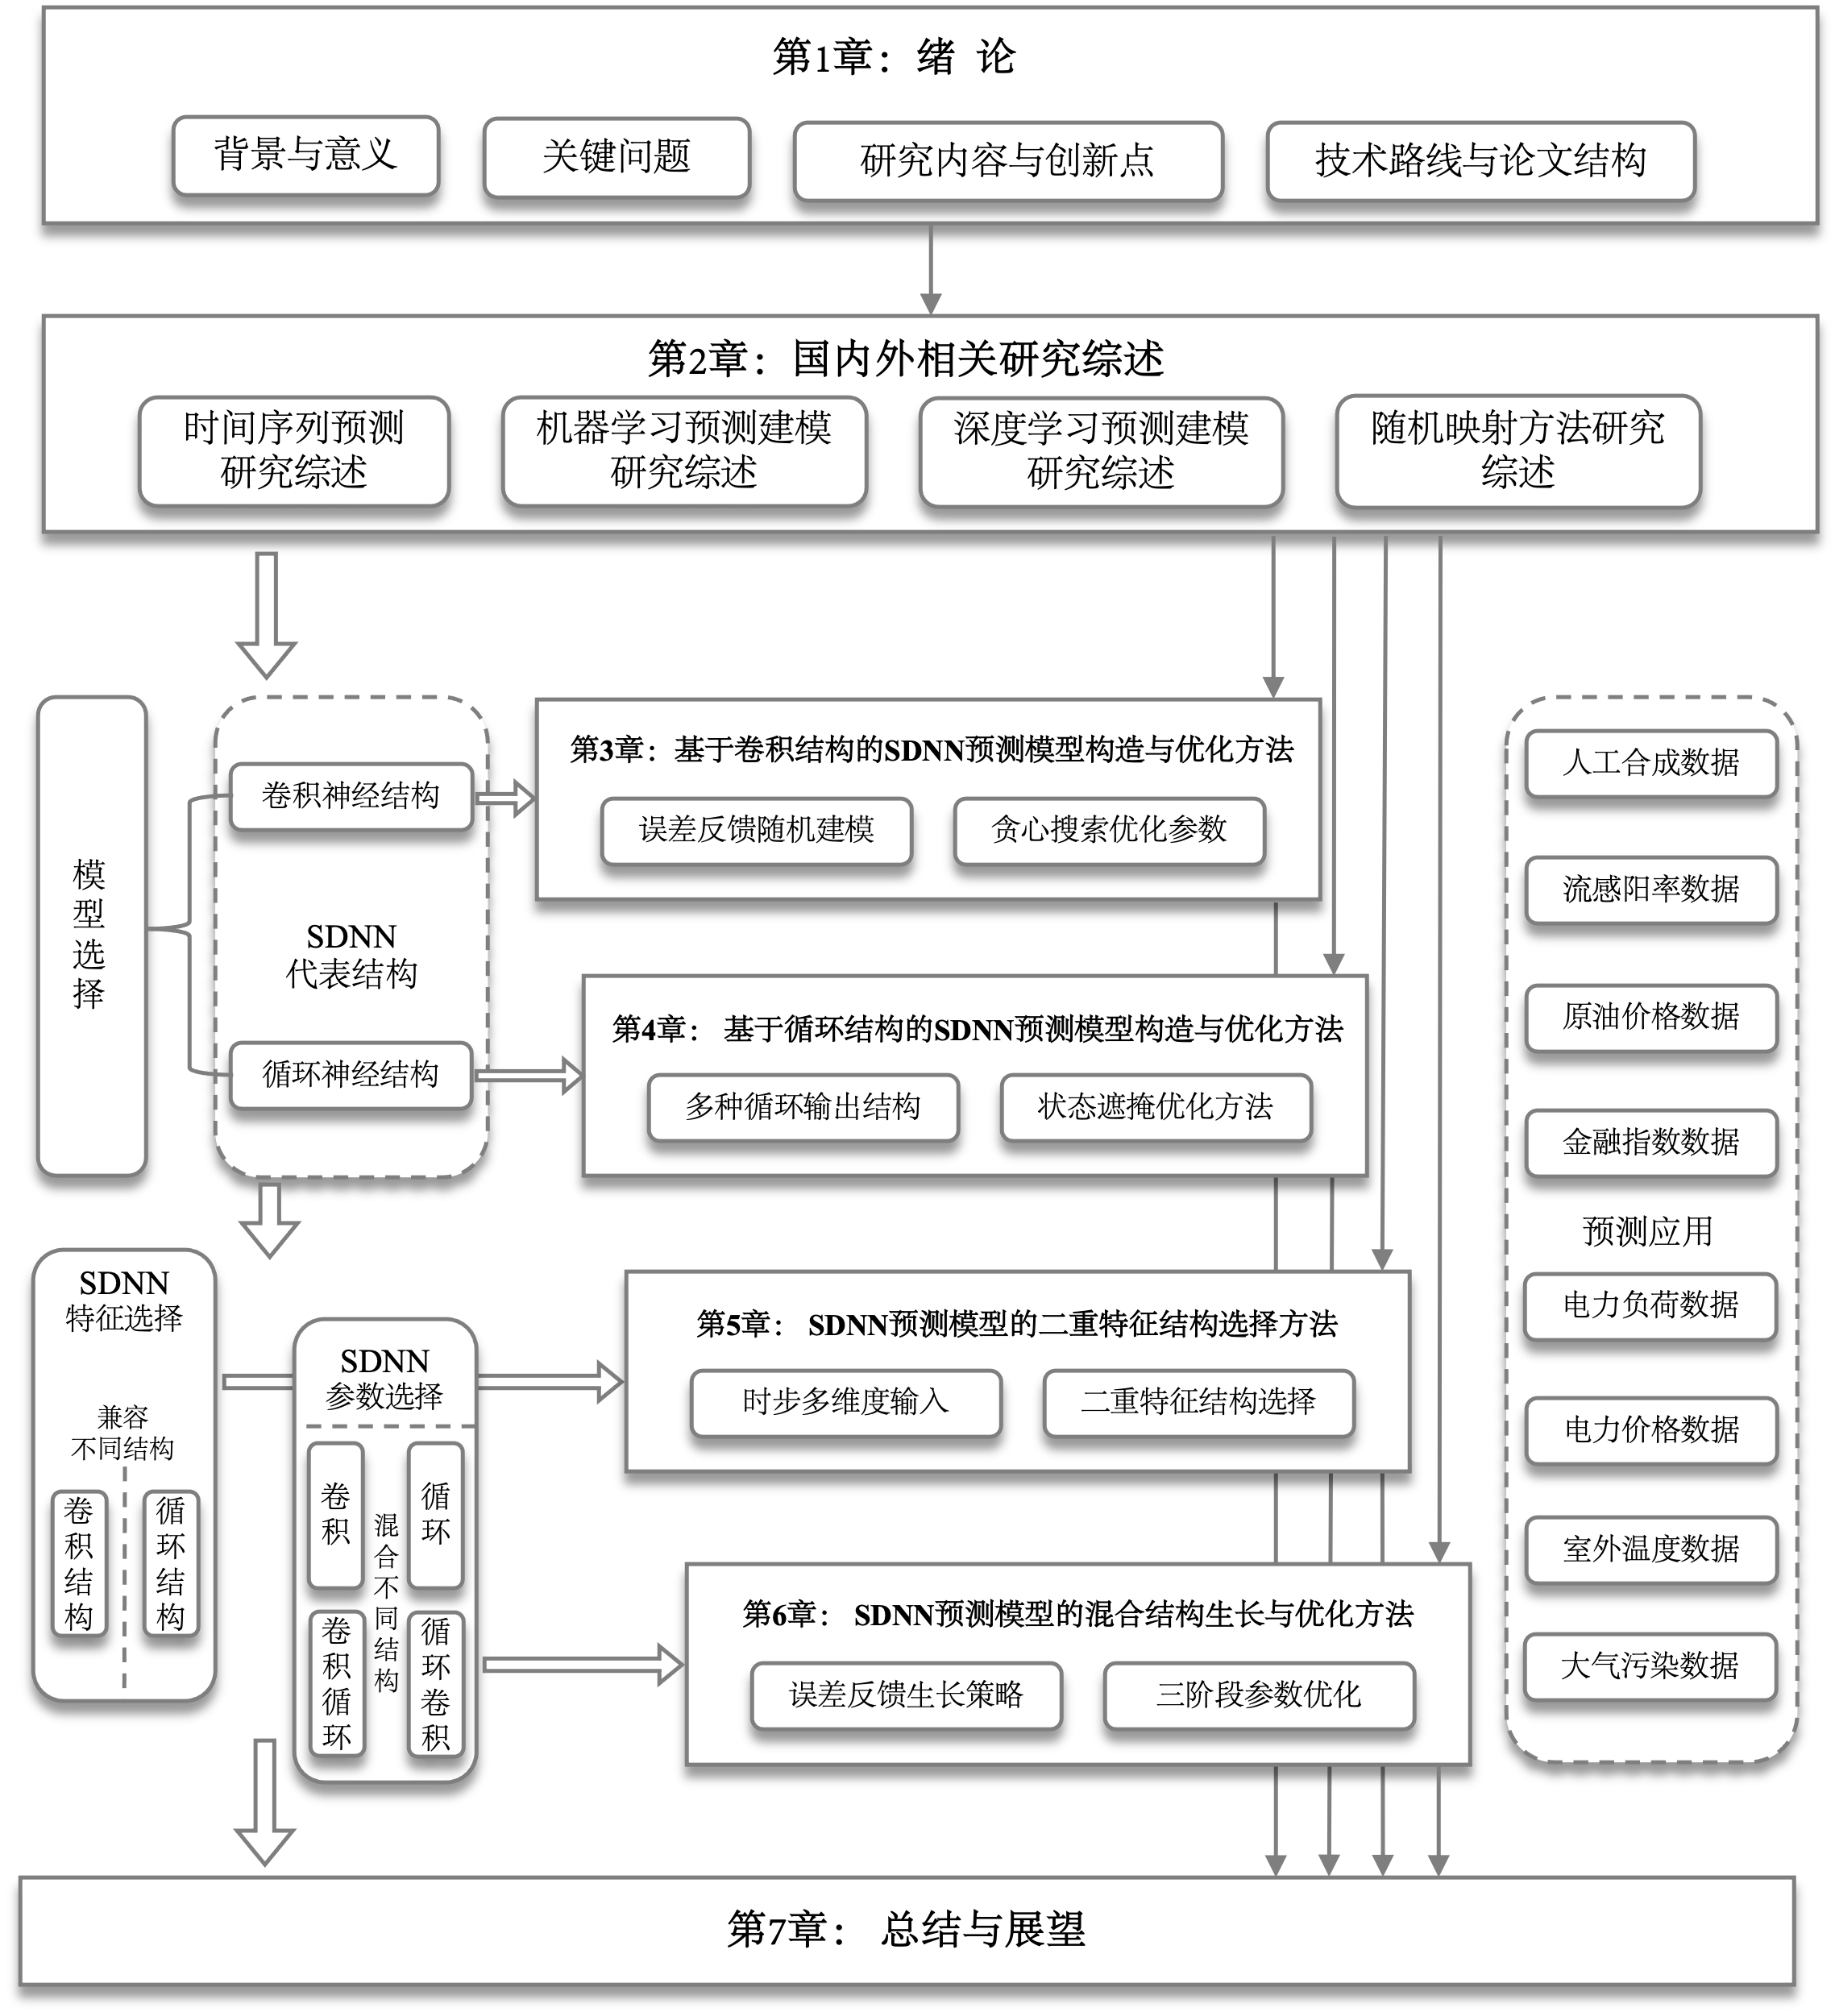
\includegraphics[width=0.9\linewidth]{float/ch.intro/thesis_content.png}
            \caption*{本论文主要结构}
        \end{minipage}

    \end{figure}
\end{frame}

\begin{frame}
    \frametitle{研究展望}
         
    卷积结构的SDNN预测模型构造与优化方法:
    \begin{itemize}
        \item 可以通过计算不同方法的时间复杂度与空间复杂度,从而精确比较各方法的建模效率优劣
        \item 基于历史数据训练和构造的模型不一定适应于时变的时间序列数据,因此可以通过考虑剪枝策略,设计模型结构对时变时间序列数据的自适应方法
    \end{itemize}

    循环结构的SDNN预测模型构造与优化方法研究
    \begin{itemize}
        \item 未有考虑状态遮掩机制对于不同随机循环隐藏结构的影响,因此可以进行状态遮掩输出结构在其他随机循环隐藏结构(如GESN或DESN结构)上的迁移实验
        \item 在梯度下降的RNN预测模型训练中同样存在类似的问题,因此可以通过设计基于状态遮掩的新颖梯度下降损失函数,提升RNN预测模型的预测效果。
    \end{itemize}

\end{frame}

\begin{frame}
    \frametitle{研究展望}
         
    SDNN预测模型的二重特征结构选择方法研究:
    \begin{itemize}
        \item 二维的时间序列输入特征结构同样适用于梯度下降训练的CNN与RNN模型,因此可以考虑进行二重特征结构选择方法在训练的深度神经网络模型上的迁移实验
        \item 可以考虑联立循环结构SDNN预测模型的输入特征时步掩码和隐藏特征时步掩码,构建多阶段整体优化的循环结构SDNN预测模型,进一步提升其预测效果
    \end{itemize}

    SDNN预测模型的混合结构生长与优化方法研究
    \begin{itemize}
        \item 限定于SDNN预测模型的输入与隐藏结构,未有考虑输出结构的生长与优化问题,因此可以构造混合多种不同输出结构的自适应端到端预测模型
        \item 随机映射方法下的误差反馈生长策略并不适用于梯度下降方法,因此可以设计基于误差反馈的子网络新颖权重训练方法,构造具有收敛保证的混合结构DNN预测模型
    \end{itemize}

\end{frame}




\begin{frame}
    \frametitle{总结与展望}

    围绕上述不足之处与改进方法,未来的研究工作将持续探索时间序列预测建模技术的更多可能与思路。
    
    希望借助随机映射方法,通过进一步的学习与交流,完善深度学习预测模型的解释性研究,探寻预测模型与其优化方法在构造选择效率与预测性能提升间的更佳平衡,使其在更为广泛的应用领域发挥可信且有效的支撑作用。


    \vspace*{1em}
    \(\circ\)衷心感谢博士生导师鲍玉昆教授、计算机科技与技术学院的何琨教授、硕士研究生导师蔡淑琴教授对我的指导。

    \(\circ\)感谢预答辩委员会的胡斌教授、王林教授、杨彦武教授和吴庆华教授。
    
    \(\circ\)感谢我的爱人、父母、朋友、师弟师妹,以及所有的支持者!

\end{frame}
